% Created by tikzDevice version 0.10.1 on 2016-02-27 13:33:59
% !TEX encoding = UTF-8 Unicode
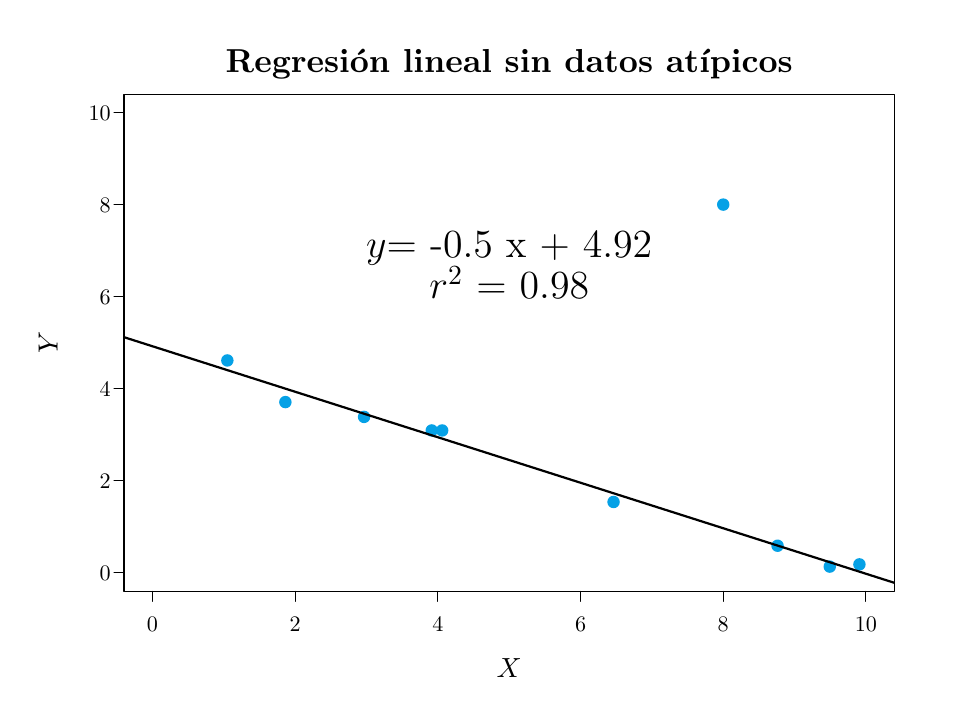
\begin{tikzpicture}[x=1pt,y=1pt]
\definecolor{fillColor}{RGB}{255,255,255}
\path[use as bounding box,fill=fillColor,fill opacity=0.00] (0,0) rectangle (325.21,238.49);
\begin{scope}
\path[clip] ( 34.80, 34.80) rectangle (313.21,214.49);
\definecolor{fillColor}{RGB}{5,161,230}

\path[fill=fillColor] ( 72.15,118.24) circle (  2.25);

\path[fill=fillColor] (270.97, 51.29) circle (  2.25);

\path[fill=fillColor] ( 93.12,103.19) circle (  2.25);

\path[fill=fillColor] (146.01, 92.94) circle (  2.25);

\path[fill=fillColor] (211.70, 67.10) circle (  2.25);

\path[fill=fillColor] (149.78, 92.94) circle (  2.25);

\path[fill=fillColor] (289.83, 43.74) circle (  2.25);

\path[fill=fillColor] (300.55, 44.55) circle (  2.25);

\path[fill=fillColor] (121.56, 97.84) circle (  2.25);
\end{scope}
\begin{scope}
\path[clip] (  0.00,  0.00) rectangle (325.21,238.49);
\definecolor{drawColor}{RGB}{0,0,0}

\path[draw=drawColor,line width= 0.4pt,line join=round,line cap=round] ( 45.11, 34.80) -- (302.90, 34.80);

\path[draw=drawColor,line width= 0.4pt,line join=round,line cap=round] ( 45.11, 34.80) -- ( 45.11, 31.21);

\path[draw=drawColor,line width= 0.4pt,line join=round,line cap=round] ( 96.67, 34.80) -- ( 96.67, 31.21);

\path[draw=drawColor,line width= 0.4pt,line join=round,line cap=round] (148.23, 34.80) -- (148.23, 31.21);

\path[draw=drawColor,line width= 0.4pt,line join=round,line cap=round] (199.79, 34.80) -- (199.79, 31.21);

\path[draw=drawColor,line width= 0.4pt,line join=round,line cap=round] (251.34, 34.80) -- (251.34, 31.21);

\path[draw=drawColor,line width= 0.4pt,line join=round,line cap=round] (302.90, 34.80) -- (302.90, 31.21);

\node[text=drawColor,anchor=base,inner sep=0pt, outer sep=0pt, scale=  0.80] at ( 45.11, 20.40) {0};

\node[text=drawColor,anchor=base,inner sep=0pt, outer sep=0pt, scale=  0.80] at ( 96.67, 20.40) {2};

\node[text=drawColor,anchor=base,inner sep=0pt, outer sep=0pt, scale=  0.80] at (148.23, 20.40) {4};

\node[text=drawColor,anchor=base,inner sep=0pt, outer sep=0pt, scale=  0.80] at (199.79, 20.40) {6};

\node[text=drawColor,anchor=base,inner sep=0pt, outer sep=0pt, scale=  0.80] at (251.34, 20.40) {8};

\node[text=drawColor,anchor=base,inner sep=0pt, outer sep=0pt, scale=  0.80] at (302.90, 20.40) {10};

\path[draw=drawColor,line width= 0.4pt,line join=round,line cap=round] ( 34.80, 41.46) -- ( 34.80,207.84);

\path[draw=drawColor,line width= 0.4pt,line join=round,line cap=round] ( 34.80, 41.46) -- ( 31.21, 41.46);

\path[draw=drawColor,line width= 0.4pt,line join=round,line cap=round] ( 34.80, 74.73) -- ( 31.21, 74.73);

\path[draw=drawColor,line width= 0.4pt,line join=round,line cap=round] ( 34.80,108.01) -- ( 31.21,108.01);

\path[draw=drawColor,line width= 0.4pt,line join=round,line cap=round] ( 34.80,141.28) -- ( 31.21,141.28);

\path[draw=drawColor,line width= 0.4pt,line join=round,line cap=round] ( 34.80,174.56) -- ( 31.21,174.56);

\path[draw=drawColor,line width= 0.4pt,line join=round,line cap=round] ( 34.80,207.84) -- ( 31.21,207.84);

\node[text=drawColor,anchor=base east,inner sep=0pt, outer sep=0pt, scale=  0.80] at ( 30.00, 38.70) {0};

\node[text=drawColor,anchor=base east,inner sep=0pt, outer sep=0pt, scale=  0.80] at ( 30.00, 71.98) {2};

\node[text=drawColor,anchor=base east,inner sep=0pt, outer sep=0pt, scale=  0.80] at ( 30.00,105.25) {4};

\node[text=drawColor,anchor=base east,inner sep=0pt, outer sep=0pt, scale=  0.80] at ( 30.00,138.53) {6};

\node[text=drawColor,anchor=base east,inner sep=0pt, outer sep=0pt, scale=  0.80] at ( 30.00,171.80) {8};

\node[text=drawColor,anchor=base east,inner sep=0pt, outer sep=0pt, scale=  0.80] at ( 30.00,205.08) {10};

\path[draw=drawColor,line width= 0.4pt,line join=round,line cap=round] ( 34.80, 34.80) --
	(313.21, 34.80) --
	(313.21,214.49) --
	( 34.80,214.49) --
	( 34.80, 34.80);
\end{scope}
\begin{scope}
\path[clip] (  0.00,  0.00) rectangle (325.21,238.49);
\definecolor{drawColor}{RGB}{0,0,0}

\node[text=drawColor,anchor=base,inner sep=0pt, outer sep=0pt, scale=  1.20] at (174.01,222.30) {\bfseries Regresión lineal sin datos atípicos};

\node[text=drawColor,anchor=base,inner sep=0pt, outer sep=0pt, scale=  1.00] at (174.01,  3.60) {$X$};

\node[text=drawColor,rotate= 90.00,anchor=base,inner sep=0pt, outer sep=0pt, scale=  1.00] at ( 10.80,124.65) {$Y$};
\end{scope}
\begin{scope}
\path[clip] ( 34.80, 34.80) rectangle (313.21,214.49);
\definecolor{fillColor}{RGB}{5,161,230}

\path[fill=fillColor] (251.34,174.56) circle (  2.25);
\definecolor{drawColor}{RGB}{0,0,0}

\path[draw=drawColor,line width= 0.8pt,line join=round,line cap=round] ( 34.80,126.65) -- (313.21, 37.88);

\node[text=drawColor,anchor=base,inner sep=0pt, outer sep=0pt, scale=  1.00] at (174.01,155.42) {\Large $y$= -0.5 x + 4.92};

\node[text=drawColor,anchor=base,inner sep=0pt, outer sep=0pt, scale=  1.00] at (174.01,140.45) {\Large $r^2$ = 0.98};
\end{scope}
\end{tikzpicture}
